\section{Project Execution}
\subsection{Phase 1 - Research and Analysis Phase}
This phase of the project is strongly managed by a research component, which would set up a framework which would support the definition and conceptual design of the e-government services and it's position in government.
Included in this phase would be the selection of a suitable government department or a predefined set of e-government services for the implementation of the solution as a pilot site. The following high level tasks have been identified. 
\slist
\spit Analysis of current requirements methodology and it's alignment to a Model Driven Approach
\spit A study would be conducted to ascertain the different types of government operational units which require e-government services
\spit Another study to provide a high-level catalog of e-services for the different types of government operational units as defined in the first phase
\spit Comparative Analysis of E-government performance
\spit Finalize Project Plan and Charter
\elist
\subsection{Phase 2 - Development Stack Design and Implementation supported by a Requirements Phase for a Given Department Type}
Once a department is selected as per phase 1, the modeling and engineering phase of the project can commence.
\slist
\spit Translate/Map the requirements to \textit{Model Types}
\spit Finalize the toolchain and ensure that the \textit{Model Types} can be supported
\elist
\subsubsection{Defining the Models} 
This phase of the project would be to define the models in order to ensure the delivery of the e-government services. Note that these models may vary in accordance with the requirements gathered in the first phase.
\slist
\spit Technical Models
\slist
\spit The Persistent Model supported by Object Relation Mapping eg. Hibernate
\spit Work-flow Models that can ESB's and jBPM
\spit Monitoring and Performance Model
\elist
\spit Domain Models \gls{DM}
\slist
\spit Business Requirements representing the Department's Model in terms of e-services
\spit Business Rules Model to ensure that the service can integrate into a department's backend infrastructure.
\elist
\elist
\subsubsection{Develop Model Engines to transform the models into executable artifacts}
The deployable artifacts would target the technology stack; the following Model Engines would be developed
\slist
\spit UI Modeling Engine - Converting the \gls{DM} into a user interface based on the graph structure; targeting multiple channels.
\spit Data Modeling Engine - Build the database artifacts including the ORM Models; optimized with caching services
\spit Business Rules Engine - Inject code into the UI, and Business Logic components of the given service to ensure compliance; Human interaction would be required
\spit Optimization Engine - Model to optimize platform; Human interaction would be required
\elist
\subsection{Phase 3 - Implementation of the Technology Infrastructure and provision of Data Infrastructure}
This phase consists primarily of the configuration of the technology stack; which would be based on opensource technologies. The main driver of this layer would be the e-services that need to be delivered by means of the \textit{Model Types}. The following objectives would be completed in this phase. 
\slist
\spit Implementation of a GUI generator for front-ends; to target multiple channels
\spit Analyze the generic components to ensure their suitability for the framework; the assumption is that these components would be used as is and a separate project would be scoped to optimize these components
\spit Design and Implement a Model Driven Online Help facility
\spit Configure and Implement Integration Service Layer
\spit Design and Implement the ORM Facilities 
\spit Configure and Implement Single-sign-on and accounting facilities
\spit Configure and implement Web-services security layer
\elist
%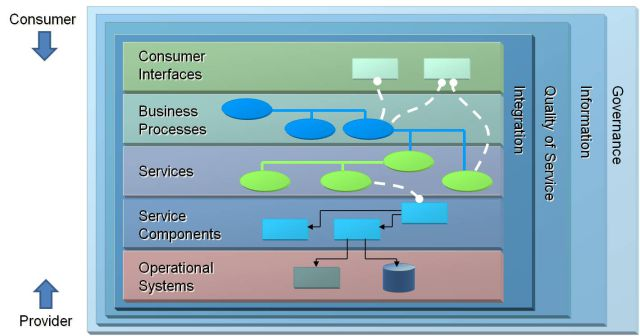
\includegraphics[width = 120mm]{images/ref-architecture.jpg}
